% Options for packages loaded elsewhere
\PassOptionsToPackage{unicode}{hyperref}
\PassOptionsToPackage{hyphens}{url}
\PassOptionsToPackage{dvipsnames,svgnames,x11names}{xcolor}
%
\documentclass[
  letterpaper,
  DIV=11,
  numbers=noendperiod]{scrartcl}

\usepackage{amsmath,amssymb}
\usepackage{iftex}
\ifPDFTeX
  \usepackage[T1]{fontenc}
  \usepackage[utf8]{inputenc}
  \usepackage{textcomp} % provide euro and other symbols
\else % if luatex or xetex
  \usepackage{unicode-math}
  \defaultfontfeatures{Scale=MatchLowercase}
  \defaultfontfeatures[\rmfamily]{Ligatures=TeX,Scale=1}
\fi
\usepackage{lmodern}
\ifPDFTeX\else  
    % xetex/luatex font selection
\fi
% Use upquote if available, for straight quotes in verbatim environments
\IfFileExists{upquote.sty}{\usepackage{upquote}}{}
\IfFileExists{microtype.sty}{% use microtype if available
  \usepackage[]{microtype}
  \UseMicrotypeSet[protrusion]{basicmath} % disable protrusion for tt fonts
}{}
\makeatletter
\@ifundefined{KOMAClassName}{% if non-KOMA class
  \IfFileExists{parskip.sty}{%
    \usepackage{parskip}
  }{% else
    \setlength{\parindent}{0pt}
    \setlength{\parskip}{6pt plus 2pt minus 1pt}}
}{% if KOMA class
  \KOMAoptions{parskip=half}}
\makeatother
\usepackage{xcolor}
\ifLuaTeX
  \usepackage{luacolor}
  \usepackage[soul]{lua-ul}
\else
  \usepackage{soul}
  
\fi
\setlength{\emergencystretch}{3em} % prevent overfull lines
\setcounter{secnumdepth}{-\maxdimen} % remove section numbering
% Make \paragraph and \subparagraph free-standing
\makeatletter
\ifx\paragraph\undefined\else
  \let\oldparagraph\paragraph
  \renewcommand{\paragraph}{
    \@ifstar
      \xxxParagraphStar
      \xxxParagraphNoStar
  }
  \newcommand{\xxxParagraphStar}[1]{\oldparagraph*{#1}\mbox{}}
  \newcommand{\xxxParagraphNoStar}[1]{\oldparagraph{#1}\mbox{}}
\fi
\ifx\subparagraph\undefined\else
  \let\oldsubparagraph\subparagraph
  \renewcommand{\subparagraph}{
    \@ifstar
      \xxxSubParagraphStar
      \xxxSubParagraphNoStar
  }
  \newcommand{\xxxSubParagraphStar}[1]{\oldsubparagraph*{#1}\mbox{}}
  \newcommand{\xxxSubParagraphNoStar}[1]{\oldsubparagraph{#1}\mbox{}}
\fi
\makeatother


\providecommand{\tightlist}{%
  \setlength{\itemsep}{0pt}\setlength{\parskip}{0pt}}\usepackage{longtable,booktabs,array}
\usepackage{calc} % for calculating minipage widths
% Correct order of tables after \paragraph or \subparagraph
\usepackage{etoolbox}
\makeatletter
\patchcmd\longtable{\par}{\if@noskipsec\mbox{}\fi\par}{}{}
\makeatother
% Allow footnotes in longtable head/foot
\IfFileExists{footnotehyper.sty}{\usepackage{footnotehyper}}{\usepackage{footnote}}
\makesavenoteenv{longtable}
\usepackage{graphicx}
\makeatletter
\def\maxwidth{\ifdim\Gin@nat@width>\linewidth\linewidth\else\Gin@nat@width\fi}
\def\maxheight{\ifdim\Gin@nat@height>\textheight\textheight\else\Gin@nat@height\fi}
\makeatother
% Scale images if necessary, so that they will not overflow the page
% margins by default, and it is still possible to overwrite the defaults
% using explicit options in \includegraphics[width, height, ...]{}
\setkeys{Gin}{width=\maxwidth,height=\maxheight,keepaspectratio}
% Set default figure placement to htbp
\makeatletter
\def\fps@figure{htbp}
\makeatother
% definitions for citeproc citations
\NewDocumentCommand\citeproctext{}{}
\NewDocumentCommand\citeproc{mm}{%
  \begingroup\def\citeproctext{#2}\cite{#1}\endgroup}
\makeatletter
 % allow citations to break across lines
 \let\@cite@ofmt\@firstofone
 % avoid brackets around text for \cite:
 \def\@biblabel#1{}
 \def\@cite#1#2{{#1\if@tempswa , #2\fi}}
\makeatother
\newlength{\cslhangindent}
\setlength{\cslhangindent}{1.5em}
\newlength{\csllabelwidth}
\setlength{\csllabelwidth}{3em}
\newenvironment{CSLReferences}[2] % #1 hanging-indent, #2 entry-spacing
 {\begin{list}{}{%
  \setlength{\itemindent}{0pt}
  \setlength{\leftmargin}{0pt}
  \setlength{\parsep}{0pt}
  % turn on hanging indent if param 1 is 1
  \ifodd #1
   \setlength{\leftmargin}{\cslhangindent}
   \setlength{\itemindent}{-1\cslhangindent}
  \fi
  % set entry spacing
  \setlength{\itemsep}{#2\baselineskip}}}
 {\end{list}}
\usepackage{calc}
\newcommand{\CSLBlock}[1]{\hfill\break\parbox[t]{\linewidth}{\strut\ignorespaces#1\strut}}
\newcommand{\CSLLeftMargin}[1]{\parbox[t]{\csllabelwidth}{\strut#1\strut}}
\newcommand{\CSLRightInline}[1]{\parbox[t]{\linewidth - \csllabelwidth}{\strut#1\strut}}
\newcommand{\CSLIndent}[1]{\hspace{\cslhangindent}#1}

\usepackage{booktabs}
\usepackage{longtable}
\usepackage{array}
\usepackage{multirow}
\usepackage{wrapfig}
\usepackage{float}
\usepackage{colortbl}
\usepackage{pdflscape}
\usepackage{tabu}
\usepackage{threeparttable}
\usepackage{threeparttablex}
\usepackage[normalem]{ulem}
\usepackage{makecell}
\usepackage{xcolor}
\KOMAoption{captions}{tableheading}
\makeatletter
\@ifpackageloaded{caption}{}{\usepackage{caption}}
\AtBeginDocument{%
\ifdefined\contentsname
  \renewcommand*\contentsname{Table of contents}
\else
  \newcommand\contentsname{Table of contents}
\fi
\ifdefined\listfigurename
  \renewcommand*\listfigurename{List of Figures}
\else
  \newcommand\listfigurename{List of Figures}
\fi
\ifdefined\listtablename
  \renewcommand*\listtablename{List of Tables}
\else
  \newcommand\listtablename{List of Tables}
\fi
\ifdefined\figurename
  \renewcommand*\figurename{Figure}
\else
  \newcommand\figurename{Figure}
\fi
\ifdefined\tablename
  \renewcommand*\tablename{Table}
\else
  \newcommand\tablename{Table}
\fi
}
\@ifpackageloaded{float}{}{\usepackage{float}}
\floatstyle{ruled}
\@ifundefined{c@chapter}{\newfloat{codelisting}{h}{lop}}{\newfloat{codelisting}{h}{lop}[chapter]}
\floatname{codelisting}{Listing}
\newcommand*\listoflistings{\listof{codelisting}{List of Listings}}
\makeatother
\makeatletter
\makeatother
\makeatletter
\@ifpackageloaded{caption}{}{\usepackage{caption}}
\@ifpackageloaded{subcaption}{}{\usepackage{subcaption}}
\makeatother

\ifLuaTeX
  \usepackage{selnolig}  % disable illegal ligatures
\fi
\usepackage{bookmark}

\IfFileExists{xurl.sty}{\usepackage{xurl}}{} % add URL line breaks if available
\urlstyle{same} % disable monospaced font for URLs
\hypersetup{
  pdftitle={Application of Spatial Monitoring and Reporting Tool (SMART) for Improving Law-Enforcement Effectiveness at Nech Sar National Park, Ethiopia.},
  pdfauthor={Zerubabel W. Demeke},
  colorlinks=true,
  linkcolor={blue},
  filecolor={Maroon},
  citecolor={Blue},
  urlcolor={Blue},
  pdfcreator={LaTeX via pandoc}}


\title{Application of Spatial Monitoring and Reporting Tool (SMART) for
Improving Law-Enforcement Effectiveness at Nech Sar National Park,
Ethiopia.}
\author{Zerubabel W. Demeke}
\date{}

\begin{document}
\maketitle


\emph{Natural Resources and the Environment Program, University of New
Hampshire.}

\emph{New Hampshire, USA.}

\emph{Zerubabel.Demeke@unh.edu}

\section{\texorpdfstring{\textbf{Abstract}}{Abstract}}\label{abstract}

\emph{Ecological monitoring is the regular observation and informing
gathering on environmental conditions with a kin purpose detect change
at different time intervals coupled with future forecasts of
environmental parameters. The Spatial Monitoring and Reporting Tool or
SMART is considered among the advanced systems for ecological
monitoring. To increase its management effectiveness, Nech Sar National
is applying the SMART approach for ecological and threat monitoring. The
Park has four patrol stations established at selected parts of the park
with due consideration for conservation requirements. The first patrol
program using the SMART CyberTracker was initiated in 2022 by deploying
56 rangers in six different teams consisting of 8 to 9 rangers per team.
In a a year long patrol; charcoal production, firewood collection, wood
logging, illegal grazing, grass cutting, illegal farming, settlement,
over fishing, and poaching were the threats recorded in the park. A
total of 10 threat types with 1,658 incidents were recorded during the
patrol. Illegal firewood collection was the highest recorded illegal
activity, followed by illegal fishing, while illegal farming was the
least recorded illegal activity. The main reasons behind the
anthropogenic pressures are identified to be the park boundary
demarcation, poor infrastructure, and low benefit-sharing schemes for
the local community.}

\textbf{Key Words:} \emph{Anthropogenic, Conservation, CyberTracker,
Ecology, Threat}

\begin{enumerate}
\def\labelenumi{\arabic{enumi}.}
\tightlist
\item
  INTRODUCTION
\end{enumerate}

SMART has evolved to become the world's leading and powerful tool in the
field of nature conservation and protected area management
(\citeproc{ref-cronin2021}{Cronin, Dancer, et al. 2021};
\citeproc{ref-wangmo2021}{Wangmo et al. 2021}). There are more than 800
National parks and other 29 conservation areas that are currently using
SMART technology in more than 70 countries around the world
(\citeproc{ref-cronin2021}{Cronin, Dancer, et al. 2021}). Although
widely recognized for being implemented at terrestrial sites, SMART can
also be readily applied to water bodies' conservation and protected area
management in which more than 50 marine sites were implementing SMART
globally (\citeproc{ref-cronin2021}{Cronin, Dancer, et al. 2021};
\citeproc{ref-gill2017}{Gill et al. 2017}). When applied to increase the
effectiveness of law enforcement, it enables the collection, storage,
communication, and evaluation of data on patrol efforts, patrol results,
and threat levels. As a result, the application of the SMART approach in
law enforcement in protected areas has been proven to reduce threats to
wildlife and natural resources at numerous sites worldwide
(\citeproc{ref-azevedo-santos2019}{Azevedo-Santos et al. 2019};
\citeproc{ref-gill2017}{Gill et al. 2017};
\citeproc{ref-huxf6tte2016}{Hötte et al. 2016}).

The first step towards achieving the goal of any biodiversity
conservation is to obtain baseline and updated information on the
biodiversity as well as existing and prospective threats
(\citeproc{ref-worku2020}{Worku and Girma 2020}). The availability of
such information on the ecological condition of the park's ecosystem,
for example, the degree of anthropogenic pressure its distribution
pattern of threats, is vital for strategic planning, and informed
decision-making. Mapping the level of each threat's hotspot area is also
essential helping to improve parks management effectiveness, by allowing
park managers to improve patrol management and threat
monitoring(\citeproc{ref-wangmo2021}{Wangmo et al. 2021}). On top of
this, the tool helps to improve patrol performance and resource
allocation and provides adaptive management decisions and patrol
deployment. Considering the challenges that park experts and rangers
face in data collection, analysis, and data management, CyberTracker and
SMART (Spatial Monitoring and Reporting Tool), are now available to
improve the effectiveness of ecological monitoring, patrol, and
site-based conservation activities on the ground
(\citeproc{ref-cronin2021a}{Cronin, Benbow, et al. 2021}).

The SMART approach for protected area has been reported to be effective
in reducing illegal activities Primorskii Krai in Russia and Marine
protected area system in Belize (\citeproc{ref-sarker2022}{Sarker and
Mahmudul Islam 2022}), Sundarbans in Bangladesh and other African
protected areas such as Cross River landscape in Nigeria, Queen
Elizabeth National Park in Uganda, Gonarezhou National Park in Zimbabwe,
North Luangwa ecosystem in Zambia Mid-Zambezi Valley
(\citeproc{ref-kavhu2021}{Kavhu and Mpakairi 2021}). Tanzania also
introduced the system in some of its game reserves (trophy hunting
areas) and national parks (\citeproc{ref-wilfred2019}{Wilfred 2019}).

Ethiopia has been establishing several protected areas since the 1960s
and has more than 179 protected areas under different categories.
However, the natural resources of the country especially the wildlife
are still facing a substantial risk of extinction, there is overgrazing
and encroachment from pastoral people, illegal human settlements,
increased extraction of fuelwood and wood logs, mineral extraction,
uncontrolled fires and extraction of other natural resources
(\citeproc{ref-husen2012}{Husen et al. 2012};
\citeproc{ref-amare2015}{Amare 2015};
\citeproc{ref-mulualem2016}{Mulualem and Tesfahunegny 2016};
\citeproc{ref-bekele2013}{K. B. Bekele 2013};
\citeproc{ref-mengist2020}{Mengist 2020}). The causes of biodiversity
loss in the country can be associated with high human population growth,
poverty, poor enforcement of existing legislation, unsustainable natural
resource management, and lack of awareness and coordination
(\citeproc{ref-bekele2018}{S. E. Bekele 2018}).

Nech Sar National Park is one of the oldest protected areas in Ethiopia
which was established in 1967 with the objective for the conservation of
the rich flora and fauna resources of the area
(\citeproc{ref-clark2010}{Clark 2010}; \citeproc{ref-jones2005}{Jones
2005}). The park with its diversified habitat types and wild animals has
immense potential as a tourist destination (\citeproc{ref-seid2019}{Seid
2019}). As Seid (2019), even if the park is rich in biodiversity, there
is a high decline in both flora and fauna population due to different
anthropogenic factors. Other scholars (\citeproc{ref-jones2005}{Jones
2005}; \citeproc{ref-clark2010}{Clark 2010};
\citeproc{ref-debelo2011}{Debelo 2011};
\citeproc{ref-aramdefetene2014}{Aramde Fetene et al. 2014}) also
highlighted the high-risk result of a persistent, diversified, and
high-level anthropogenic pressure: natural resource extraction.

Protected areas administration in Ethiopia is divided into two
categories, some are managed by the Ethiopian Wildlife Conservation
Authority at the Federal level and others are under the administration
of regional states. However, all the parks, whether under federal or
regional state administration, have different and unstandardized
monitoring systems with due limitations in regular and continuous data
for informed decision-making. On top of that, park managers don't have a
mechanism to measure management effectiveness or evaluate patrol
performance and efficiency. As a result, the SMART approach for
ecological and threat monitoring was introduced in 2019, and Nech Sar
National Park used SMART CyberTracker as a standard system to conduct
its regular wildlife surveys, habitat, and threat monitoring.

\begin{enumerate}
\def\labelenumi{\arabic{enumi}.}
\setcounter{enumi}{1}
\item
  METHODOLOGY

  2.1. The SMART Approach
\end{enumerate}

SMART version 5.0.3 integrated with the CyberTracker application was
used by installing the software on a dedicated desktop computer for the
task. The technical training manual for SMART 5.0.3, guides, and other
materials found at \url{http://smartconservationtools.org} were used and
the default data model was then customized in a way that reflects the
situations of the park (Figure 1), configured and transferred to the
CyberTracker application on smartphones. CyberTracker operates within a
GPS-enabled mobile device i.e., a smartphone or a Personal Digital
Assistant (PDA) to collect observation and GPS data in a single unit.
With a proper setup including patrol details, conservation area profile,
and other related information.

\begin{figure}[H]

{\centering \includegraphics{images/Fig1.png}

}

\caption{The customized SMART data model of Nech Sar National Park}

\end{figure}%

2.2 Patrol Framework and Design

As an adaptive management approach, ranger-based monitoring and
conservation area management leveraging SMART are based on point
observations and track logs generated by ranger patrols. These logs are
entered into a database and analyzed to produce data summaries and
reports, which are thenfed back to ranger teams as patrol plans (Figure
2).

\begin{figure}[H]

{\centering \includegraphics{images/Picture2.png}

}

\caption{Nech Sar National Park Patrol framework}

\end{figure}%

SMART was designed to facilitate each step in this cycle:~

\ul{Step 1:} Data Collection; Patrol teams collect and record data on
where they go and what they see while on patrol, including threats
(e.g., charcoal production and firewood collection), and the actions
taken (e.g., arrests, confiscations of materials). These data are
collected on smartphones equipped with the CyberTracker application,
standardizing and simplifying data collection, and adding increased
efficiency and transparency.~

\ul{Step 2}: Data Entry; Patrol teams report their patrol activities,
followed by patrol data and routes that are checked and then stored in
the SMART database. Since the park is using smartphones for data
collection, the process is automated, eliminating data entry errors.

\ul{Step 3}: Analysis, and Reporting; data are then processed
semi-automatically into user-defined, highly visual tables, charts, and
maps showing patrol effort, coverage, and results, forming the basis for
patrol and trend analysis and rapid evaluation.

\ul{Step 4:} Feedback and Evaluation; regular meetings with rangers are
held to discuss patrol effort and results to ensure all stakeholders are
kept informed and to demonstrate the value of ranger efforts.

\ul{Step 5}: Strategic Planning; managers, rangers, and other
stakeholders then plan adaptive patrol strategies based on analysis of
previous results, changing conditions, and/or temporal patterns, and set
new patrol targets.

2.3. Data Collection

A total of four patrol stations or ranger outposts were established by
dividing the park into different zones for better success of management
interventions. Boundaries of the patrol stations were defined based on
the understanding of the conservation requirements of Nech Sar National
Park and principal ecosystem components. After providing intensive
training on the application of SMART CyberTracker focusing on how to
operate the CyberTracker application and data recording. The patrol was
conducted by deploying rangers in six different teams where each patrol
team shifts to a different patrol station every month. A total of six
patrolling teams consisting of 8 to 9 rangers participated in the patrol
and each team had a team leader the total number of rangers involved
during the law enforcement operation was 56 including one chief ranger
leader assigned to each team.

2.4. Data Analysis

The illegal threats were grouped into their categories and attributes
were then semi-analyzed by SMART (Spatial Monitoring and Reporting
Tools) 5.0.3 versions software by directly downloading the field data
from the CyberTracker application used to collect the data using android
smart phones. The semi-analyzed data on SMART then exported in Excel
format where further analysis is conducted by Rstudio (R 4.4.1). The
types of illegal threats, distribution, the patrol effort of each team,
encounter rates, and action taken to threats are also analyzed. The
results are then presented by simple statistical tools like figures,
tables, and charts.

\begin{enumerate}
\def\labelenumi{\arabic{enumi}.}
\setcounter{enumi}{2}
\tightlist
\item
  RESULTS
\end{enumerate}

3.1. Types and Trends of Conservation Threats in NSNP

In the illegal violations monitoring many threats to the National Park
were identified. Of Charcoal production, Firewood collection, and Grass
collection were the most observed ones followed by illegal fishing,
illegal grazing, wood logging, and grass cutting. Charcoal production
and waste disposal incidents were medium encounter rate categories
during patrol missions. On the other hand, Wildlife Hunting, Illegal
farming, and Settlement incidents were the lowest encounter rate
category during patrol missions.

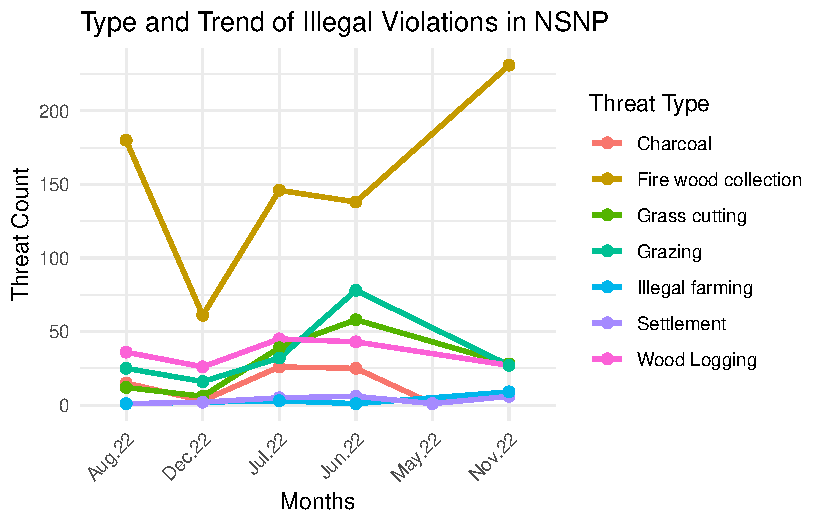
\includegraphics{Final_files/figure-pdf/unnamed-chunk-1-1.pdf}

3.2. The Origin and Sex Ratio of Illegal Entry to the Park

3.2.1. The Origin of Illegal Entry to the Park

Nech Sar National Park (NSNP) currently facing severe conservation
threats due to high Illegal entry to the park. In the present patrol,
914 incidents from Arba Minch Zuria Woreda followed by Arba Minch town
and Guji Commity inside the park, 256 and 213, respectively. On the
other hand, fewer incidents of illegal entry from Gamo Zone and
surrounding Zone and Woreda such as Dita Woreda, Gerese Woreda, Chencha
Woreda, Kuch Woreda, Kemba Woreda, Wolaita Zone, Kore Community, Boreda
Woreda, Gofa Zone, Basket Special Woreda on the illegal fishing
activity,~Gacho Baba Woreda.

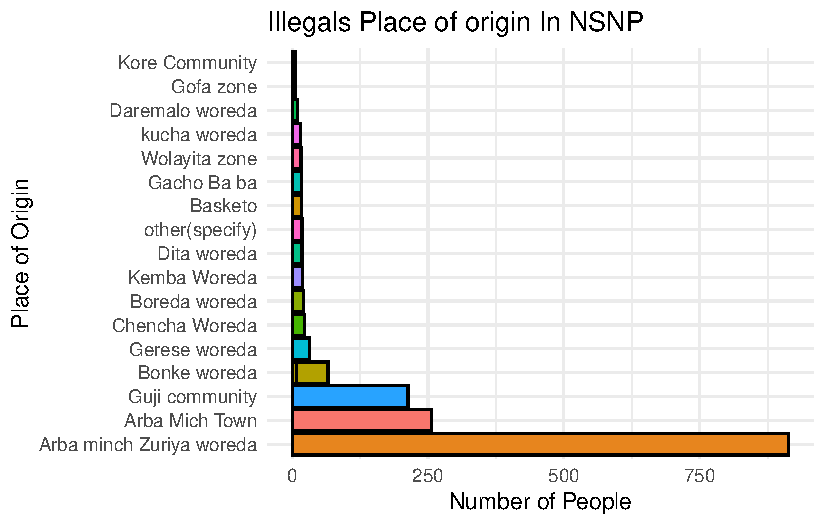
\includegraphics{Final_files/figure-pdf/unnamed-chunk-2-1.pdf}

3.2.2. Sex Ratio of Illegal Entry

The sex category of illegal entry to the National Park is given in
Figure 7. A total of 1,658 illegal entries were observed during patrol
time. ~Overall, 980 males (59.1\%), 647 females (39\%), and 31 unknown
sex (1.9\%) or hidden by bushy and natural barriers, respectively.

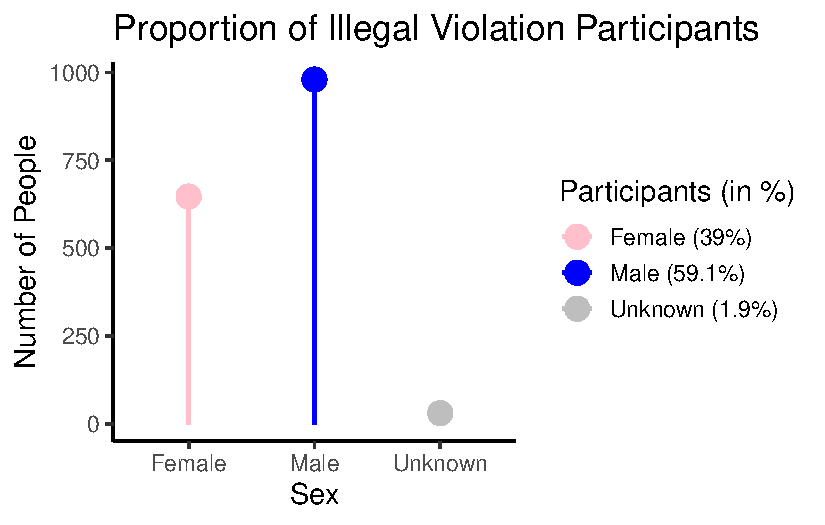
\includegraphics{Final_files/figure-pdf/unnamed-chunk-3-1.pdf}

3.3. Patrol Effort and Team Performance of Rangers

Nech Sar National Park has 56 rangers in the park, stationed on four
different outposts. Each outpost has a monthly changing team of eight to
nine members or teams with one additional team leader for each team.
Their responsibilities are patrolling the park and, as a result, the
patrol team's performance by number of days, distance walked by km,
Active Patrol Hours, Distance (km) per number of Days, and Number of
Active Patrol Hours per number of Days.

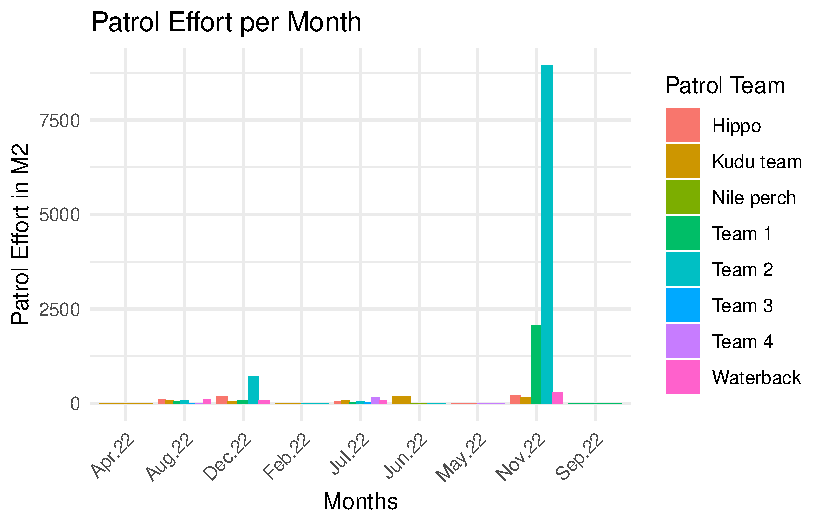
\includegraphics{Final_files/figure-pdf/unnamed-chunk-4-1.pdf}

Table 1 shows the summary queries, showing patrol effort or performance
for individual Rangers (Note: the table shown from a SMART report from
which the names of rangers have been removed and replaced by Ranger1 up
to Ranger 6) While the graph below indicates the an area covered by
patrol teams.

\begin{longtable}[t]{lrrrrr}
\caption{Patrol Effort and Team Performance}\\
\toprule
Patrol.Team & No.of.Days & Distance..km. & Active.Hours & Distance..Day & Active.Hours.Day\\
\midrule
Ranger1 & 95 & 1017.6 & 470.1 & 10.7 & 4.9\\
Ranger2 & 96 & 1606.3 & 689.2 & 16.7 & 7.2\\
Ranger3 & 65 & 891.6 & 415.1 & 13.7 & 6.4\\
Ranger4 & 67 & 1182.5 & 508.7 & 17.6 & 7.6\\
Ranger5 & 71 & 1118.7 & 527.5 & 15.7 & 7.4\\
\addlinespace
Ranger6 & 57 & 618.9 & 353.0 & 10.8 & 6.2\\
\bottomrule
\end{longtable}

\begin{enumerate}
\def\labelenumi{\arabic{enumi}.}
\setcounter{enumi}{4}
\tightlist
\item
  DISCUSSION
\end{enumerate}

Charcoal production, Firewood collection, Wood logging, illegal grazing,
Grass cutting, illegal farming and Settlement, Overfishing, and illegal
poaching were the major threats to Nech Sar National Park. Conservation
challenges of Park and major threats are resulted from human
encroachment that ranked in the result (Figure 1). Although 1,656
illegal entries were observed/recorded during the current study time
(2022) other field research results indicate 457 in 2017
(\citeproc{ref-alemu2017}{Alemu 2017}), 265 in 2015
(\citeproc{ref-nsnp2015}{NSNP 2015}), and 147 in 2012
(\citeproc{ref-fetene2012}{Fetene, Bekele, and Tiwari 2012}) that
reflect an increase on conservation threats.

Arba Minch groundwater forest lowland riverine forest within Nech Sar
National Park is one of the few remaining forest areas in Ethiopia and
has been suffering from a high degree of deforestation as local
townspeople cut the trees for subsistence and the people of Arba Minch
town who rely on wood for cooking. In the park, 20 hectares of the
forest coverage has been cleared (cut) for firewood collection and
charcoal production, and 6 hectares of forest are cleared annually,
according to the park's ecological survey report, 2018 E.C
(\citeproc{ref-nsnp2018}{NSNP 2018}). Similarly, other reports support
the ecological report of the park, indicating a high pressure on natural
forests (\citeproc{ref-aregu2006}{Aregu and Demeke 2006})showcasing
units of parks such as forestland, grassland, and wooded grassland to be
the most threatened habitat types (\citeproc{ref-fetene2016}{Fetene et
al. 2016}). Human encroachment or interference by Guji pastoralists
living inside and around the park and firewood collectors, pole cutters,
charcoal makers, and fishermen (\citeproc{ref-genayetsegaye2017}{Genaye
Tsegaye et al. 2017})has also intensified the problem.

The massive number of livestock herds present in the park augmented by
seasonal migration which competes with the inadequate available feed in
the wet season will take the predominant role in the decline of the
herbivore mammals in the plain of the park. The natural resources
depletion resulted from livestock grazing and other anthropogenic
pressures related decline in the number of wild animals, in Nech Sar
National Park (\citeproc{ref-shibru2020}{Shibru et al. 2020}), adjacent
to the Gamabela National Park (\citeproc{ref-seidmoh}{{``Seid Mohammed
and Taye Behailu (2018). Public Attitude... - Google Scholar,''} n.d.})
Chebera Churchura National Park, Ethiopia
(\citeproc{ref-megaze2017}{Megaze, Balakrishnan, and Belay 2017}), and
Awash, Yangudi Rassa and Aledeghi National Park; where a population of
cattle, sheep, and goats of the pastoralist are flooding in these
protected areas. This also leads to wildlife being stressed by
disturbance, and shortage of food (\citeproc{ref-wale2017}{Wale et al.
2017}). The Illegal Farmland expansion and settlement in the northeast
of the park have been utilizing the resource in an unsustainable way for
short-term benefit without considering the longer-term impact
(\citeproc{ref-abiyot2009}{Abiyot 2009}).

\begin{enumerate}
\def\labelenumi{\arabic{enumi}.}
\setcounter{enumi}{4}
\tightlist
\item
  CONCLUSION AND RECOMMENDATION
\end{enumerate}

Both urban and rural communities are largely dependent on forest
resources for firewood and construction or as a business option to
support their family's daily livelihood demands. The other
park-threatening pressure is livestock grazing, expansion of settlement
and illegal farming, and poaching, particularly in the Eastern parts of
the park. On the other hand, more than a significant number of people
with their cattle live within the park. Anthropogenic threats to the
National Park's biodiversity include charcoal production, firewood
collection, wood logging, illegal grazing, grass cutting, illegal
farming and settlement, overfishing, and illegal poaching, etc. Besides,
disagreement on the park boundary, ecosystem degradation, habitat loss,
low infrastructure (roads and eco-tourism center), and low benefit of
the local community from the park are the major causes of illegal
threats.

As it's possible to understand from the results, Improving
infrastructure, facilities, and field equipment (roads, campsites, post
sites, information centers) will contribute to reducing illegal
violations and promote effective management. On the other hand,
developing sustainable~ benefit sharing schemes and alternative means to
support the livelihood of communities also enhances the sustainable
conservation of the park. Developing awareness of the community and
respective role of them and other stakeholders~can also develop a sense
of ownership for the community and other stakeholders.

\begin{enumerate}
\def\labelenumi{\arabic{enumi}.}
\setcounter{enumi}{4}
\tightlist
\item
  REFERENCES
\end{enumerate}

\phantomsection\label{refs}
\begin{CSLReferences}{1}{0}
\bibitem[\citeproctext]{ref-abiyot2009}
Abiyot, Negera. 2009. {``Resettlement and Local Livelihoods in Nechsar
National Park, Southern Ethiopia.''} \emph{Unpublished MPhil Thesis,
University of Tromsø}.

\bibitem[\citeproctext]{ref-alemu2017}
Alemu, Molla Mekonnen. 2017. {``The Paradigm of Fuelwood Consumption
Around National Parks and Its Implication for National Policies: The
Case of Nech Sar National Park, Ethiopia.''} \emph{Open Access Library
Journal} 4 (02): 1. \url{https://www.scirp.org/html/73951_73951.htm}.

\bibitem[\citeproctext]{ref-amare2015}
Amare, Alemneh. 2015. {``Wildlife Resources of Ethiopia: Opportunities,
Challenges and Future Directions: From Ecotourism Perspective: A Review
Paper.''} \emph{Natural Resources} 6 (6): 405422.
\url{https://www.scirp.org/journal/paperinformation?paperid=57447}.

\bibitem[\citeproctext]{ref-aramdefetene2014}
Aramde Fetene, Aramde Fetene, Kumelachew Yeshitela Kumelachew Yeshitela,
Ruediger Prasse, and Thomas Hilker. 2014. {``Study of Changes in Habitat
Type Distribution and Habitat Structure of Nech Sar National Park,
Ethiopia.''}
\url{https://www.cabidigitallibrary.org/doi/full/10.5555/20153156350}.

\bibitem[\citeproctext]{ref-aregu2006}
Aregu, Lemlem, and Fassil Demeke. 2006. {``Socio-Economic Survey of
Arba-Minch Riverine Forest and Woodland.''} \emph{Journal of the
Drylands} 1 (2): 194205.

\bibitem[\citeproctext]{ref-azevedo-santos2019}
Azevedo-Santos, Valter M., Renata G. Frederico, Camila K. Fagundes,
Paulo S. Pompeu, Fernando M. Pelicice, André A. Padial, Marcos G.
Nogueira, et al. 2019. {``Protected Areas: A Focus on Brazilian
Freshwater Biodiversity.''} Edited by Robert Cowie. \emph{Diversity and
Distributions} 25 (3): 442--48. \url{https://doi.org/10.1111/ddi.12871}.

\bibitem[\citeproctext]{ref-bekele2013}
Bekele, Kibruyisfa Berihun. 2013. {``Attitudes on the Correlation of the
Academic Achievement and Physical Proficiency: The Case of Top Ten
Natural Science Preparatory Students in Each Section, at Lideta Sub-City
in Addis Ababa.''} PhD thesis.
\url{http://thesisbank.jhia.ac.ke/id/eprint/5293}.

\bibitem[\citeproctext]{ref-bekele2018}
Bekele, Solomon Estifanos. 2018. {``Parkland Agroforestry of Ethiopia;
Key to Production, Productivity, Biodiversity Conservation and Climate
Change Mitigation: A Review.''} \emph{Open Journal of Forestry} 08 (04):
472. \url{https://doi.org/10.4236/ojf.2018.84030}.

\bibitem[\citeproctext]{ref-clark2010}
Clark, Derek L. 2010. \emph{An Introduction to the Natural History of
Nech Sar National Park}. Ethiopian Wildlife \& Natural History Society.

\bibitem[\citeproctext]{ref-cronin2021a}
Cronin, Drew T., Sophie Benbow, Richard A. Bergl, Liz Bourgault, Lina
Caro, Anthony Dancer, Alasdair Davies, et al. 2021. {``Empowering
Rangers Through Technology and Innovation.''} \emph{Parks Stewardship
Forum} 37 (1). \url{https://doi.org/10.5070/P537151750}.

\bibitem[\citeproctext]{ref-cronin2021}
Cronin, Drew T., Anthony Dancer, Barney Long, Antony J. Lynam, Jeff
Muntifering, Jonathan Palmer, Richard A. Bergl, S. A. Wich, and A. K.
Piel. 2021. {``Application of SMART Software for Conservation Area
Management.''} \emph{Conservation Technology}, 203223.
\url{https://books.google.com/books?hl=en&lr=&id=DHo8EAAAQBAJ&oi=fnd&pg=PA201&dq=Drew+T.+Cronin,+Anthony+Dancer,+Barney+Long,+Antony+J.+Lynam,+Jeff+Muntifering,+Jonathan+Palmer,+and+Richard+A.+Berg+(2021).Application+of+SMART+software+for+conservation+area+managements.+In:+Conservat:on++DOI:+10.1093/oso/9780198850243.003.0010&ots=3PBMZSouXm&sig=qUcjgie3rxwLxP73_9d4efWfZWs}.

\bibitem[\citeproctext]{ref-debelo2011}
Debelo, Asebe Regassa. 2011. {``Contested Terrains: Conflicts Between
State and Local Communities over the Management and Utilization of Nech
Sar National Park, Southern Ethiopia.''} \emph{Journal of Sustainable
Development in Africa} 13 (5): 4965.
\url{https://jsd-africa.com/Jsda/Vol13No5_Fall2011_A/PDF/Contested\%20terrains.pdf}.

\bibitem[\citeproctext]{ref-fetene2012}
Fetene, Aramde, Tsegaye Bekele, and P. K. Tiwari. 2012. {``Impact of
Human Activities on Ground Water Forests of Arba Minch: A Case Study
from Ethiopia.''} \emph{International Journal of Basic and Applied
Sciences} 1 (1): 5460.
\url{https://www.academia.edu/download/30585777/4_IJBAS__2012__1(1)__54-60.pdf}.

\bibitem[\citeproctext]{ref-fetene2016}
Fetene, Aramde, Thomas Hilker, Kumelachew Yeshitela, Ruediger Prasse,
Warren Cohen, and Zhiqiang Yang. 2016. {``Detecting Trends in Landuse
and Landcover Change of Nech Sar National Park, Ethiopia.''}
\emph{Environmental Management} 57: 137147.
\url{https://idp.springer.com/authorize/casa?redirect_uri=https://link.springer.com/article/10.1007/s00267-015-0603-0&casa_token=X2actQ-JEIAAAAAA:krtIWQi51IWOjPUQg9CbffuV3OKjCq6Vv_N2IoJ9tG5m1GnGJmggTnoYU_oVM4JF8M6PH2-dnLaV2oSK}.

\bibitem[\citeproctext]{ref-genayetsegaye2017}
Genaye Tsegaye, Genaye Tsegaye, S. Dondeyne, Mulugeta Lemenih Mulugeta
Lemenih, Abraham Marye Abraham Marye, J. Nyssen, J. A. Deckers, and M.
Maertens. 2017. {``'Facing Conservation'or'conservation with a Human
Face'? People-Park Interactions in Southern Ethiopia.''}
\url{https://www.cabidigitallibrary.org/doi/full/10.5555/20173252372}.

\bibitem[\citeproctext]{ref-gill2017}
Gill, David A., Michael B. Mascia, Gabby N. Ahmadia, Louise Glew, Sarah
E. Lester, Megan Barnes, Ian Craigie, Emily S. Darling, Christopher M.
Free, and Jonas Geldmann. 2017. {``Capacity Shortfalls Hinder the
Performance of Marine Protected Areas Globally.''} \emph{Nature} 543
(7647): 665669.
\url{https://idp.nature.com/authorize/casa?redirect_uri=https://www.nature.com/articles/nature21708&casa_token=DmpBnRpR3OoAAAAA:RL3FkrbqcDF1qIOGNkcqzXcfU3WxbDZZwTkYRa45LaMekd3os0lTXzIkD6w4MQjzOoSxX1R0YtbDBjaf}.

\bibitem[\citeproctext]{ref-huxf6tte2016}
Hötte, Michiel H. H., Igor A. Kolodin, Sergei L. Bereznuk, Jonathan C.
Slaght, Linda L. Kerley, Svetlana V. Soutyrina, Galina P. Salkina, Olga
Y. Zaumyslova, Emma J. Stokes, and Dale G. Miquelle. 2016. {``Indicators
of Success for Smart Law Enforcement in Protected Areas: A Case Study
for Russian Amur Tiger ( {\emph{Panthera Tigris Altaica}} ) Reserves.''}
\emph{Integrative Zoology} 11 (1): 2--15.
\url{https://doi.org/10.1111/1749-4877.12168}.

\bibitem[\citeproctext]{ref-husen2012}
Husen, Azamal, V. K. Mishra, Kamal Semwal, and Dinesh Kumar. 2012.
{``Biodiversity Status in Ethiopia and Challenges.''}
\emph{Environmental Pollution and Biodiversity} 1: 3179.
\url{https://www.researchgate.net/profile/Azamal-Husen/publication/258049236_Biodiversity_Status_in_Ethiopia_and_Challenges/links/5a87e96c458515b8af8df732/Biodiversity-Status-in-Ethiopia-and-Challenges.pdf}.

\bibitem[\citeproctext]{ref-jones2005}
Jones, Alison M. 2005. {``A Proposed Management Plan for Ethiopia{'}s
Nech Sar National Park.''} \emph{CONTEXT} 4: 13.
\url{https://alisonjonesphoto.com/NGOs/NSNP-paper-3-4-06-lowres.pdf}.

\bibitem[\citeproctext]{ref-kavhu2021}
Kavhu, Blessing, and Kudzai Shaun Mpakairi. 2021. {``Spatial Monitoring
and Reporting Tool (SMART) in Mid{-}Zambezi Valley, Zimbabwe:
Implementation Challenges and Practices.''} \emph{Conservation Science
and Practice} 3 (9): e492. \url{https://doi.org/10.1111/csp2.492}.

\bibitem[\citeproctext]{ref-megaze2017}
Megaze, Aberham, Mundanthra Balakrishnan, and Gurja Belay. 2017. {``The
Attitudes and Practices of Local People Towards Wildlife in Chebera
Churchura National Park, Ethiopia.''} \emph{International Journal of
Biodiversity and Conservation} 9 (2): 4555.
\url{https://academicjournals.org/journal/IJBC/article-full-text/4699BE962717}.

\bibitem[\citeproctext]{ref-mengist2020}
Mengist, W. 2020. {``Challenges of Protected Area Management and
Conservation Strategies in Ethiopia: A Review Paper.''} \emph{Adv.
Environ. Stud} 4: 277285.
\url{https://www.academia.edu/download/107746556/aes-4-029.pdf}.

\bibitem[\citeproctext]{ref-mulualem2016}
Mulualem, Getachew, and Weldemariam Tesfahunegny. 2016. {``Review of Key
Wildlife Threats Factors from Literature and Observation Perspectives: A
Way Forward for Sustainable Wildlife Genetic Resource Conservation
Practices in Ethiopia.''} \emph{The Journal of Zoology Studies} 3 (5):
0112.
\url{https://scholar.archive.org/work/tycxc7z47bewhbibnc4uswscje/access/wayback/http://www.journalofzoology.com:80/archives/volume3/issue5/PartA/1.1.pdf}.

\bibitem[\citeproctext]{ref-nsnp2015}
NSNP. 2015. {``Nech Sar National Park, 2015 Annual Report.''}

\bibitem[\citeproctext]{ref-nsnp2018}
---------. 2018. {``Nech Sar National Park, 2018 Annual Report.''}

\bibitem[\citeproctext]{ref-sarker2022}
Sarker, Subrata, and M. Mahmudul Islam. 2022. {``Marine Protected Area
and Biodiversity Conservation.''} In, edited by Walter Leal Filho,
Anabela Marisa Azul, Luciana Brandli, Amanda Lange Salvia, and Tony
Wall, 629--44. Cham: Springer International Publishing.
\url{https://link.springer.com/10.1007/978-3-319-98536-7_127}.

\bibitem[\citeproctext]{ref-seid2019}
Seid, Mohammed. 2019. {``Critical Solutions for Critical Problems:
Threats to Sustainable Use and Management of Nech Sar National Park
(NSNP) in Ethiopia.''} \url{https://philpapers.org/rec/SEICSF}.

\bibitem[\citeproctext]{ref-seidmoh}
{``Seid Mohammed and Taye Behailu (2018). Public Attitude... - Google
Scholar.''} n.d.
\url{https://scholar.google.com/scholar?hl=en&as_sdt=0\%2C30&q=Seid+Mohammed+and+Taye+Behailu+\%282018\%29.+Public+attitude+and+prospective+factors+of+wildlife+conservation+the+case+of+Gambela+National+Park\%2C+Southwest+Ethiopia.+International+Journal+of+Advanced+Research+in+Biological+Sciences+ISSN\%3A+2348-8069.+DOI\%3A+10.22192\%2Fijarbs&btnG=}.

\bibitem[\citeproctext]{ref-shibru2020}
Shibru, Simon, Karen Vancampenhout, Jozef Deckers, and Herwig Leirs.
2020. {``Human Pressure Threaten Swayne{'}s Hartebeest to Point of Local
Extinction from the Savannah Plains of Nech Sar National Park, South
Rift Valley, Ethiopia.''} \emph{Journal of Biodiversity and Endangered
Species} 8 (1): 8.
\url{https://www.researchgate.net/profile/Simon-Shibru/publication/339927093_Human_Pressure_Threaten_Swayne's_Hartebeest_to_Point_of_Local_Extinction_from_the_Savannah_Plains_of_Nech_Sar_National_Park_South_Rift_Valley_Ethiopia/links/5e6c7840299bf12e23c35646/Human-Pressure-Threaten-Swaynes-Hartebeest-to-Point-of-Local-Extinction-from-the-Savannah-Plains-of-Nech-Sar-National-Park-South-Rift-Valley-Ethiopia.pdf}.

\bibitem[\citeproctext]{ref-wale2017}
Wale, Mengistu, Abeje Kassie, Getachew Mulualem, Weldemariam
Tesfahunegny, and Abraham Assefa. 2017. {``Wildlife Threats and Their
Relative Severity of Eastern Ethiopia Protected Areas.''} \emph{Ecology
and Evolutionary Biology} 2 (4): 5967.
\url{https://www.academia.edu/download/86664595/10.11648.j.eeb.20170204.12.pdf}.

\bibitem[\citeproctext]{ref-wangmo2021}
Wangmo, Singye, Sonam Wangdi, Alexander Wyatt, Kuenley Tenzin, Jampel
Lhendup, and Rohit Singh. 2021. {``Driven by Data: Improved Protected
Area Effectiveness in Royal Manas National Park, Bhutan.''}
\emph{Conservation Science and Practice} 3 (10): e503.
\url{https://doi.org/10.1111/csp2.503}.

\bibitem[\citeproctext]{ref-wilfred2019}
Wilfred, Paulo. 2019. {``The Challenges Facing Resident Hunting in
Western Tanzania: The Case of the Ugalla Ecosystem.''} \emph{European
Journal of Wildlife Research} 65 (6): 86.

\bibitem[\citeproctext]{ref-worku2020}
Worku, Zerubabel, and Zerihun Girma. 2020. {``Large Mammal Diversity and
Endemism at Geremba Mountain Fragment, Southern Ethiopia.''}
\emph{International Journal of Ecology} 2020 (April): 1--11.
\url{https://doi.org/10.1155/2020/3840594}.

\end{CSLReferences}




\end{document}
